% 第 9 周交付物：在线架构设计、性能基线与 GARCH 锚定对照（中文版）—— 编译方式：XeLaTeX
\documentclass[11pt]{ctexart}
\usepackage[a4paper, margin=2.2cm]{geometry}
\usepackage{amsmath, amssymb}
\usepackage{booktabs}
\usepackage{graphicx}
\usepackage{float}
\usepackage[hidelinks]{hyperref}
\usepackage{enumitem}
\setlist{nosep}
\usepackage{parskip}

\title{\textbf{在线架构设计、性能基线与 GARCH 锚定对照}\\
\large Chooser Option 定价项目 · 第 9 周（Enhancement 第 1 周）}
\author{佟铸城（Zhucheng Tong）}
\date{2026 年 9 月 22 日}

\begin{document}
\maketitle

\section{本周目标与完成情况}

Enhancement 阶段的第一周承担"搭骨架"的任务：把前八周的文件式研究原型改造成可持续在线运行的服务，并为后三周（股票池扩充、性能优化）准备好度量尺子。导师确认的边界：内网 Docker 具备在线能力即可，不做云部署；性能只看相对提升；理论线并行。

\begin{center}\small
\begin{tabular}{p{4.0cm}p{11.0cm}}
\toprule
目标 & 完成情况 \\
\midrule
PostgreSQL 与 Redis 跑通 & 9 张表的模式（多股票就绪）、迁移脚本、文件数据回填；Redis 缓存层带无缓存降级 \\
JPM 单票全链路 & 采集 $\to$ 入库 $\to$ 特征 $\to$ 报价 $\to$ 缓存 $\to$ 前端读库，联网增量更新实测 4.5 秒 \\
调度器 & APScheduler，每个交易日 17:30（纽约时间）自动运行；\texttt{--once} 手动触发 \\
一键部署 & \texttt{docker compose up -d --build}（PostgreSQL、Redis、迁移、应用、调度器五个容器）；无 Docker 的开发机用 \texttt{scripts/dev\_services.sh} 复现同一套服务 \\
性能基线 & 11 个环节的时间与内存留档（优化前），含硬件信息 \\
理论线 & GARCH(1,1) 期限结构锚定与 EWMA 锚定在 oracle 面板上对照 \\
自检 & 八项在线栈审计全部通过；第 7 周六项工具审计仍全部通过 \\
\bottomrule
\end{tabular}
\end{center}

\section{架构}

\subsection{组件与数据流}

\begin{center}\small
\begin{tabular}{p{1.9cm}p{4.6cm}p{8.6cm}}
\toprule
组件 & 实现 & 职责 \\
\midrule
持久层 & PostgreSQL 16，SQLAlchemy Core & 原始行情、指数、利率、特征、每日报价、情景表、模型登记、运行日志 \\
热数据层 & Redis 7，\texttt{src/cache} & 报价与情景表按（标的、日期、参数、模型版本）键缓存，TTL 1 小时；流水线写库后按标的失效；Redis 不可达时自动降级为直接计算 \\
服务层 & \texttt{src/tool/}\newline\texttt{pricing\_service.py} & 定价逻辑唯一所在；\texttt{load\_market\_state} 优先读库、无库时读文件，两条路径同一套算术 \\
流水线 & \texttt{src/service/pipeline.py} & 增量采集（上次日期前推 10 天重叠，幂等 upsert）$\to$ 重建特征 $\to$ 报价 $\to$ 写库 $\to$ 失效缓存 $\to$ 记日志 \\
调度器 & \texttt{src/service/scheduler.py} & APScheduler cron，工作日收盘后触发流水线 \\
前端 & \texttt{app/streamlit\_app.py} & 薄壳，零公式；新增"运行状态"页签展示表行数、运行日志与缓存命中 \\
编排 & \texttt{docker-compose.yml} & 五个服务，健康检查与启动顺序（迁移完成后再起应用与调度器） \\
\bottomrule
\end{tabular}
\end{center}

数据流：Yahoo Finance / FRED $\to$ \texttt{prices\_daily} / \texttt{index\_daily} / \texttt{rates\_daily} $\to$ \texttt{src/features}（第 2 周算术的通用化版本）$\to$ \texttt{features\_daily} $\to$ 服务层（EWMA 锚、ML 参考价、误差带）$\to$ \texttt{quotes\_daily} / \texttt{scenarios\_daily} $\to$ Redis $\to$ 前端。

\subsection{表结构}

所有市场表带 \texttt{ticker} 列，第 10 周扩股票池不需要改表。

\begin{center}\small
\begin{tabular}{p{3.0cm}p{4.0cm}p{7.8cm}}
\toprule
表 & 主键 & 内容 \\
\midrule
securities & ticker & 标的清单、所属股票池、是否活跃 \\
prices\_daily & (ticker, date) & OHLCV、复权收盘、股息、拆股、来源 \\
index\_daily & (symbol, date) & \^{}VIX、\^{}GSPC、\^{}TNX、\^{}IRX \\
rates\_daily & date & DGS3MO、DGS1、DGS10、FEDFUNDS、T10Y2Y \\
features\_daily & (ticker, date) & 收盘、复权收盘、VIX 与 18 个特征（通用列名） \\
quotes\_daily & (ticker, date) & 主定价、误差带、ML 参考价、两腿、$\sigma$、$r$、$q$、状态、模型版本 \\
scenarios\_daily & (ticker, date, scenario) & 八个极端情景的价格与变化 \\
model\_registry & name & 部署模型路径、SHA-256、角色 \\
pipeline\_runs & id & 每次运行的起止时间、状态、各表写入行数、错误信息 \\
\bottomrule
\end{tabular}
\end{center}

\subsection{设计决策}

\begin{itemize}
  \item \textbf{特征算术抽成通用模块}：第 2 周的 \texttt{preprocess.py} 针对 JPM 列名写死；第 9 周把算术移入 \texttt{src/features.py}（通用列名），文件管道通过重命名调用同一函数。审计 1 证明两种表示逐位一致，第 3--8 周的所有脚本无需改动。
  \item \textbf{文件路径保留为回退}：未配置 \texttt{DATABASE\_URL} 时服务层自动读第 2 周文件，前八周全部脚本照常运行；GitHub Actions 周更管道保留作独立备份。
  \item \textbf{幂等写入}：所有写库走 \texttt{INSERT ... ON CONFLICT DO UPDATE}，流水线可重复运行；增量采集带 10 天重叠区以吸收数据源对近期数据的修订。
  \item \textbf{缓存失效由写入方负责}：流水线写库后立即删除该标的的全部键，缓存的陈旧上限就是数据刷新间隔。
  \item \textbf{文件回填只做引导，不覆盖}：回填脚本对已有行 \texttt{ON CONFLICT DO NOTHING}，联网流水线才有覆盖权。这条规则来自容器实跑暴露的一个缺陷：文件快照末尾有一条收盘价为空的残缺行，回填把它覆盖回库后，滚动窗口特征在其后全部变为 NaN，参考模型拒绝输入。现在残缺行在写入前被丢弃，服务层也只选取全部特征完整的最新一行。
  \item \textbf{模型版本入库}：每条报价记录生成它的模型版本与登记表中的 SHA-256，第 6 周"测试集开封一次"的模型不会被静默替换。
\end{itemize}

\subsection{部署与运行}

\begin{center}\small
\begin{tabular}{p{6.6cm}p{8.2cm}}
\toprule
命令 & 作用 \\
\midrule
\texttt{docker compose up -d --build} & 首次启动：建表、回填文件数据、重算报价，然后起前端与调度器 \\
\texttt{docker compose logs -f scheduler} & 观察每日任务 \\
\texttt{bash scripts/dev\_services.sh start} & 无 Docker 的开发机：源码编译的 PostgreSQL 与 Redis \\
\texttt{python -m src.db.migrate; python -m src.db.ingest} & 建表与回填 \\
\texttt{python -m src.service.pipeline [--dry-run]} & 手动跑一次流水线（\texttt{--dry-run} 不联网，只重算） \\
\texttt{python -m src.service.scheduler --once} & 手动触发调度任务 \\
\bottomrule
\end{tabular}
\end{center}

说明：compose 栈已在 Docker Desktop 29.7 上实跑：五个容器启动、迁移与回填成功、容器内联网流水线成功、容器内八项审计全部通过、容器内报价与本机逐位一致。本机 PostgreSQL 与 Redis（\texttt{dev\_services.sh}）与容器映射同一组端口，二者不可同时运行。依赖版本已在 \texttt{requirements.txt} 精确钉死（首次构建时 pip 解析到 scikit-learn 1.9 与 pandas 3.0，而部署模型由 1.7.1 序列化，必须一致）。

\section{在线栈审计（八项，全部通过）}

\begin{center}\small
\begin{tabular}{p{0.8cm}p{7.4cm}p{6.6cm}}
\toprule
编号 & 断言 & 结果 \\
\midrule
1 & 库中特征 == 文件特征（JPM，排除末尾 15 天数据源修订窗口） & 2170 个交易日，最大差 $5.7\times10^{-14}$，NaN 模式一致 \\
2 & 库路径报价 == 文件路径报价（同一 as-of 日，全部价格字段） & 最大差 $2.3\times10^{-13}$ \\
3 & 缓存命中 == 重新计算；情景表一致；失效后键被删除 & 通过 \\
4 & 流水线幂等：重算两次，报价表行数与数值不变 & 通过 \\
5 & 库中每条报价可由同日特征重算复现 & 最大差 0 \\
6 & 迁移幂等：建表两次，表集合固定 & 9 张表 \\
7 & 前端零公式、只引用服务/缓存/仓储层 & 通过（第 7 周审计 6 的扩展） \\
8 & 调度触发器合法，下一次触发为工作日 17:30 纽约时间 & 通过 \\
\bottomrule
\end{tabular}
\end{center}

审计 1 的修订窗口来自一个真实发现：联网流水线重拉最近 10 天后，文件快照末尾两个交易日的利率、VIX 与 Parkinson 波动率与库中不同。查证后是 FRED 与 Yahoo 对近期数据的正常修订，而非计算差异。

\section{性能基线（优化前）}

按导师要求，后续只报告相对提升，本表是"优化前"的留档。硬件：Apple M4 Pro（14 核）、24 GB 内存、macOS 26.3、Python 3.13.5；每项重复 5 次取中位数，内存为 tracemalloc 峰值。

\begin{center}\small
\begin{tabular}{p{0.9cm}p{7.2cm}rr}
\toprule
编号 & 环节 & 中位耗时 & 峰值内存 \\
\midrule
S1 & 服务层冷导入（新解释器） & 477.5 ms & -- \\
S2 & 特征历史加载：CSV 文件 / PostgreSQL & 4.1 / 27.9 ms & 1.0 / 3.2 MB \\
S3 & 市场状态推导（EWMA 与利率偏差） & 0.6 ms & 0.5 MB \\
S4 & 单次报价，第 7 周路径（每次重读模型文件） & 2.2 ms & 12.6 MB \\
S5 & 单次报价，第 9 周路径（模型常驻） & 1.8 ms & 0.01 MB \\
S6 & 单次报价，Redis 命中 & 0.15 ms & -- \\
S7 & 情景表：计算 / Redis 命中 & 0.59 / 0.20 ms & -- \\
S8 & 面板定价 1310 天：标量循环 / 向量化闭式解 & 344.7 / 0.32 ms & -- \\
S9 & 重算流水线（不联网：特征重建、写库、报价） & 1935 ms & 48.3 MB \\
S10 & 每日流水线（联网，13 个新交易日） & 4498 ms & -- \\
S11 & Streamlit 首屏渲染（无头模式） & 724 ms & 28.7 MB \\
\bottomrule
\end{tabular}
\end{center}

进程末态常驻内存 366 MB；数据库 11.1 MB（2185 个交易日）；特征 CSV 756 KB；Redis 1.0 MB。

\textbf{读数}：
\begin{itemize}
  \item 单次报价与情景表都在毫秒级，前端交互不是瓶颈；Redis 把报价从 1.8 ms 压到 0.15 ms，单票场景下收益有限，多票概览页签才会体现。
  \item 库读比文件慢 7 倍（28 对 4 ms），是每次请求都拉整段历史重算 EWMA 所致；把 \texttt{sigma\_ewma} 与 \texttt{r\_1y\_dev} 落库、只读最后一行是明确的优化点。
  \item 面板定价的标量循环比向量化慢约 1000 倍。第 10 周 500 只股票的批量日更若沿用逐票标量报价，会成为最大瓶颈；向量化闭式解已经存在（第 4 周），需要把服务层的批量路径接上。
  \item 重算流水线 1.9 秒里大头是每天重建并写回全部 2185 行特征。改为只重算受滚动窗口影响的末尾 252 行并增量写入，预计缩短一个数量级。
  \item 冷导入 0.48 秒中大部分来自 torch 与 shap 的导入，服务层并不需要它们，可延迟导入。
\end{itemize}
这五条即第 12 周优化的候选清单，届时以本表为分母报告倍数。

\section{理论线：GARCH(1,1) 期限结构锚定}

\subsection{动机}

工具的主定价把 EWMA（$\lambda=0.94$）作为波动率锚。EWMA 是 GARCH(1,1) 在 $\omega=0$、$\alpha+\beta=1$ 时的退化形式：一个没有均值回复的积分过程。一年期 chooser 需要的是期权\textbf{存续期内}的平均波动率，与之在理论上匹配的锚是 GARCH 的期限结构预测
\[
\sigma_{1y}^2=\frac{1}{H}\sum_{k=1}^{H}\mathbb{E}_t[h_{t+k}],\qquad
\mathbb{E}_t[h_{t+k}]=v+(\alpha+\beta)^{k-1}\,(h_{t+1}-v),\quad v=\frac{\omega}{1-\alpha-\beta},\ H=252,
\]
它把当前方差沿存续期向长期水平回复。本周的问题是：这个理论匹配的锚，是否比经验锚 EWMA 把逐日 ATM chooser 定得更接近事后真值。

\subsection{协议}

沿用第 4 周的 oracle 面板与第 4 周的 8 指标加权综合分（参照 EWMA，$<1$ 即胜）。参数每 21 个交易日在截至当日的全部收益上重估（扩展窗，至少 750 个观测），两次重估之间用已估参数逐日滤波，不用任何未来信息。候选：GARCH 1 年期限结构锚、GARCH 1 日锚（下一日方差年化）、252 日已实现波动率；参照：EWMA。面板 1011 个交易日（2020-12-23 至 2024-12-31，比第 4 周短是因为首个 GARCH 估计需要 750 个观测），69 次重估，持续性 $\alpha+\beta$ 均值 0.955（0.934--0.972）。

\subsection{结果}

\begin{center}\footnotesize
\begin{tabular}{lrrrrrrrr}
\toprule
锚 & MAE(\$) & RMSE & Bias & P95AE & 最差状态 MAE & $R^2$ & Hit10 & 综合分 \\
\midrule
EWMA（参照） & 6.29 & 8.05 & $-1.61$ & 14.38 & 6.66 & $-0.10$ & 25.0\% & 1.000 \\
GARCH 1 日 & 5.56 & 7.71 & $-0.53$ & 13.78 & 5.86 & $-0.01$ & 31.9\% & 0.852 \\
\textbf{GARCH 1 年期限结构} & \textbf{4.18} & \textbf{5.25} & $+3.43$ & \textbf{10.09} & \textbf{4.85} & \textbf{0.53} & \textbf{46.1\%} & \textbf{0.804} \\
252 日已实现 & 7.72 & 10.24 & $+1.04$ & 27.09 & 7.96 & $-0.77$ & 23.8\% & 1.276 \\
\bottomrule
\end{tabular}
\end{center}

四种权重方案（主权重、等权、精度导向、稳健导向）下 GARCH 1 年锚均排第一。分状态：平静期 MAE 4.85 对 EWMA 6.66，恐慌期 1.66 对 4.89。分年：2021 年 3.70 对 6.48，2022 年 2.72 对 3.86，2024 年 2.27 对 9.40；\textbf{2023 年反而更差}，7.95 对 5.36。

\begin{figure}[H]
\centering
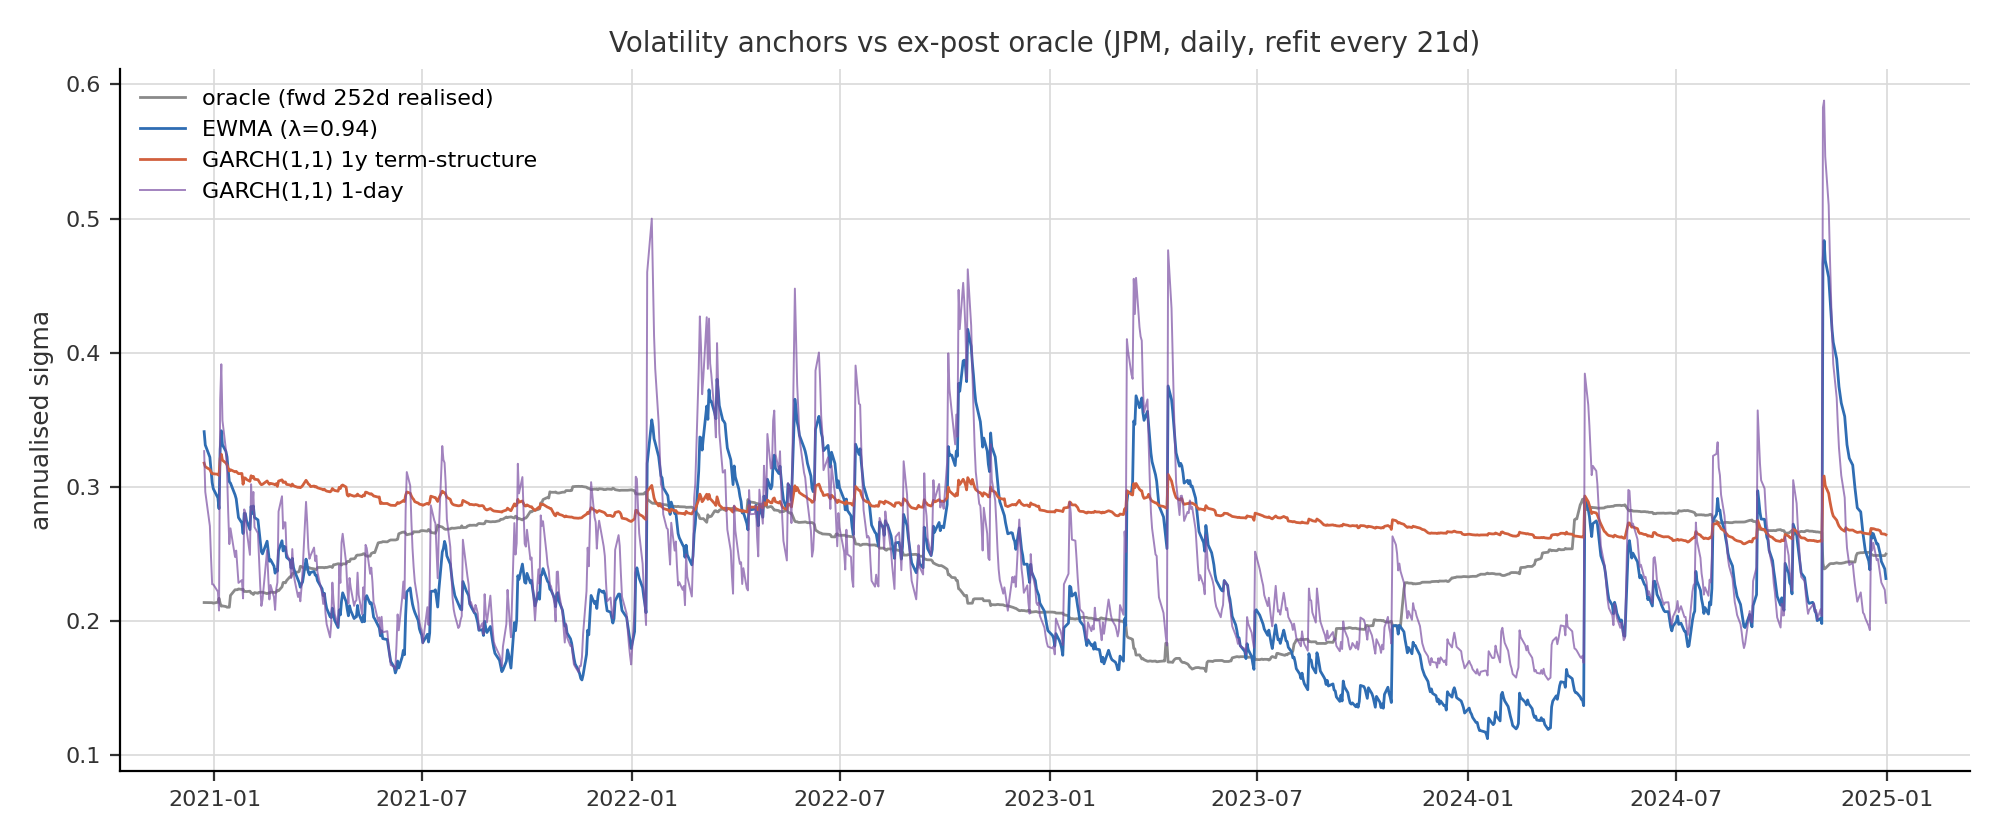
\includegraphics[width=0.94\textwidth]{figures/garch_vs_ewma.png}
\caption{三个锚与事后真值：GARCH 1 年锚（橙）几乎是一条围绕长期水平的平线，EWMA（蓝）与 GARCH 1 日锚（紫）追逐每一次尖峰}
\end{figure}

\begin{figure}[H]
\centering
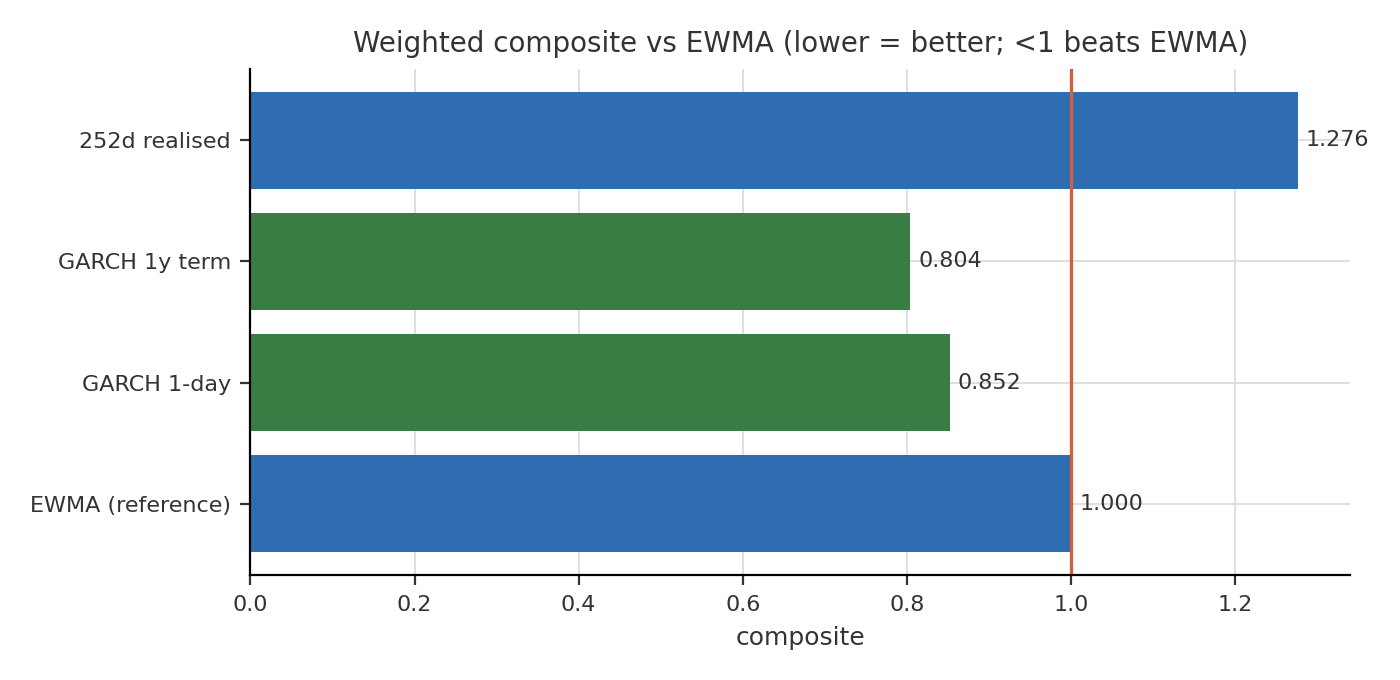
\includegraphics[width=0.62\textwidth]{figures/garch_composite.png}
\caption{加权综合分（参照 EWMA = 1）}
\end{figure}

\subsection{读数与保留意见}

\begin{enumerate}
  \item \textbf{赢在不追尖峰，而不是赢在预测}。图 1 说明 1 年锚几乎等于长期方差水平（0.27--0.31），$H=252$ 的平均把持续性 0.95 的均值回复几乎做满。它的优势集中在尾部指标（P95AE 10.1 对 14.4）与 $R^2$（0.53 对 $-0.10$）：EWMA 在恐慌日把一年期的 $\sigma$ 抬到 0.4 以上，而真值从未超过 0.31。这与第 4 周"快估计器恐慌期追高失效"的发现是同一件事的另一面。
  \item \textbf{代价是正偏差}。Bias $+3.43$ 美元：长期水平由包含 2020 年的扩展窗估出，在 2023 年这种持续平静期系统性高估，当年 MAE 反而比 EWMA 差 2.6 美元。一个偏高的常数在这段样本里恰好比一个追涨杀跌的估计器更接近真值，这不等于它是更好的预测器。
  \item \textbf{单一标的、单一区间}。本周只是 JPM 的 1011 天，与第 5 周"验证集曾胜"的教训相同：一次胜利不构成部署证据。第 10 周把同一协议放到 S\&P 500 面板上，看它是否跨股票、跨状态稳定，才决定是否把工具的锚从 EWMA 换成 GARCH 期限结构，或把它作为第 6 周锚定残差学习的新锚。
  \item \textbf{与随机过程分工的一致性}。这条线没有引入机器学习，只是把锚从"经验平滑"换成"理论匹配的期限结构"，属于最终报告第 7 章分工中"随机过程管框架"的一侧；若它在面板上站住，ML 残差学习的起点会更干净。
\end{enumerate}

\section{第 10 周衔接}

工程线：股票池扩到 S\&P 500 历史成分股（多源轮换与限流应对），调度器上线，前端加标的选择与概览页签，批量定价走向量化路径。理论线：GARCH 期限结构锚在 S\&P 500 面板上复检；锚定残差 ML 第一轮（walk-forward、测试集封存）。

\end{document}
